\chapter{Effect of Operating Systems on Results}

In this chapter, we present an observation made while evaluating our proposed
scheduler, namely the simulation results varied depending on the operating
system it was run. First, in Sec.~\ref{sec:effect} the effect of our observation
on measured performance metrics is shown. Afterwards the result of conducted
numerical experiments to investigate possible reasons for different OS behavior
is given in Sec.~\ref{sec:experiments}

\section{Overview} \label{sec:effect}

All simulations for this thesis were performed on a NCS software framework
implemented in C++\footnotemark. During the course of evaluation, we have
discovered numerical inconsistencies in measured network average
$\overline{MSE}$ and AoI $\overline{\Delta}$ among simulations performed on
Linux, Mac and Windows platforms. For reproducibility, Tab.~(\ref{tab:specs})
lists specification for the used computing systems. It should be pointed out
that FHS and GES evaluations in Ch.~\ref{ch:evaluation} were performed on Linux,
while simulation on Mac and Windows were conducted for this chapter's
investigation.

\begin{table}[b]
  \begin{center}
  \begin{tabular}{|l|c|c|>{\centering\arraybackslash}p{3.4cm}|} 
  \hline
  \textbf{Environment} & \textbf{Linux} & \textbf{Mac} & \textbf{Windows} \\
  \hline \hline
  Compiler & g++ 8.4.0 & Apple clang 11.0.0 & g++ 10.2.0 (Mingw-w64) \\ 
  Operating System & Ubuntu 18.04.05 & macOS 10.15.7 & Windows 10 Ver. 1809 \\ 
  % Kernel & GNU/Linux 4.15.0-117-generic x86\_64 & x86\_64-apple-darwin19.6.0 & WIN32 \\ 
  CPU & Intel Xeon E5-2690v2 & Intel Core i5-4260U & Intel Core i5-4670 \\
  % Cores & 32 & 4 & 4 \\
  \hline
  \end{tabular}
  \caption[Summary of runtime environment for tested simulation
  platforms]{Summary of runtime environment for tested simulation platforms.
  Note that Mingw-64 is a port of the GNU Compiler Collection (GCC) for
  Windows.}
  \label{tab:specs}
  \end{center}
\end{table}

To make the investigation more tractable, we replace the GE model with a simpler
channel model. As reference case, the setting from \cite{ayan2020aoi} is taken,
which utilizes the base FH scheduler. Here, $N=3$ heterogenous NCSs with system
matrices $A_i\in\left\{1.0, 1.25, 1.5 \right\}$ share a lossy wireless channel
with i.i.d normal packet loss, i.e., $p_i(t) \sim \mathcal{N}(0.3,0.2)$. 

Fig.~(\ref{fig:observation}) illustrates our findings for measured
$\overline{MSE}$ and $\overline{\Delta}$ for varying finite horizon $H=\left\{1,
\dots, 9\right\}$ over 200 simulation runs. We can examine the same decreasing
trend for both metrics on all OSs. However, the absolute deviations are quite
significant. In particular, the estimation error at Horizon $H=1$ deviate
between Windows and Linux for almost 50\%. On the other hand, between Mac and
Linux a consistent difference of roughly 20\% for MSE and 2\% for AoI is
observed. In contrast, the Windows $\overline{MSE}$ trajectory starts following
the Mac trajectory until $H=5$, and continues to progress along the Linux
trajectory afterwards. For network average AoI $\overline{\Delta}$, the Windows
trajectory does not follow a specific OS but rather progresses individually.

\begin{figure}[htb]
  \centering
  \begin{subfigure}[b]{0.49\textwidth}
    \centering
    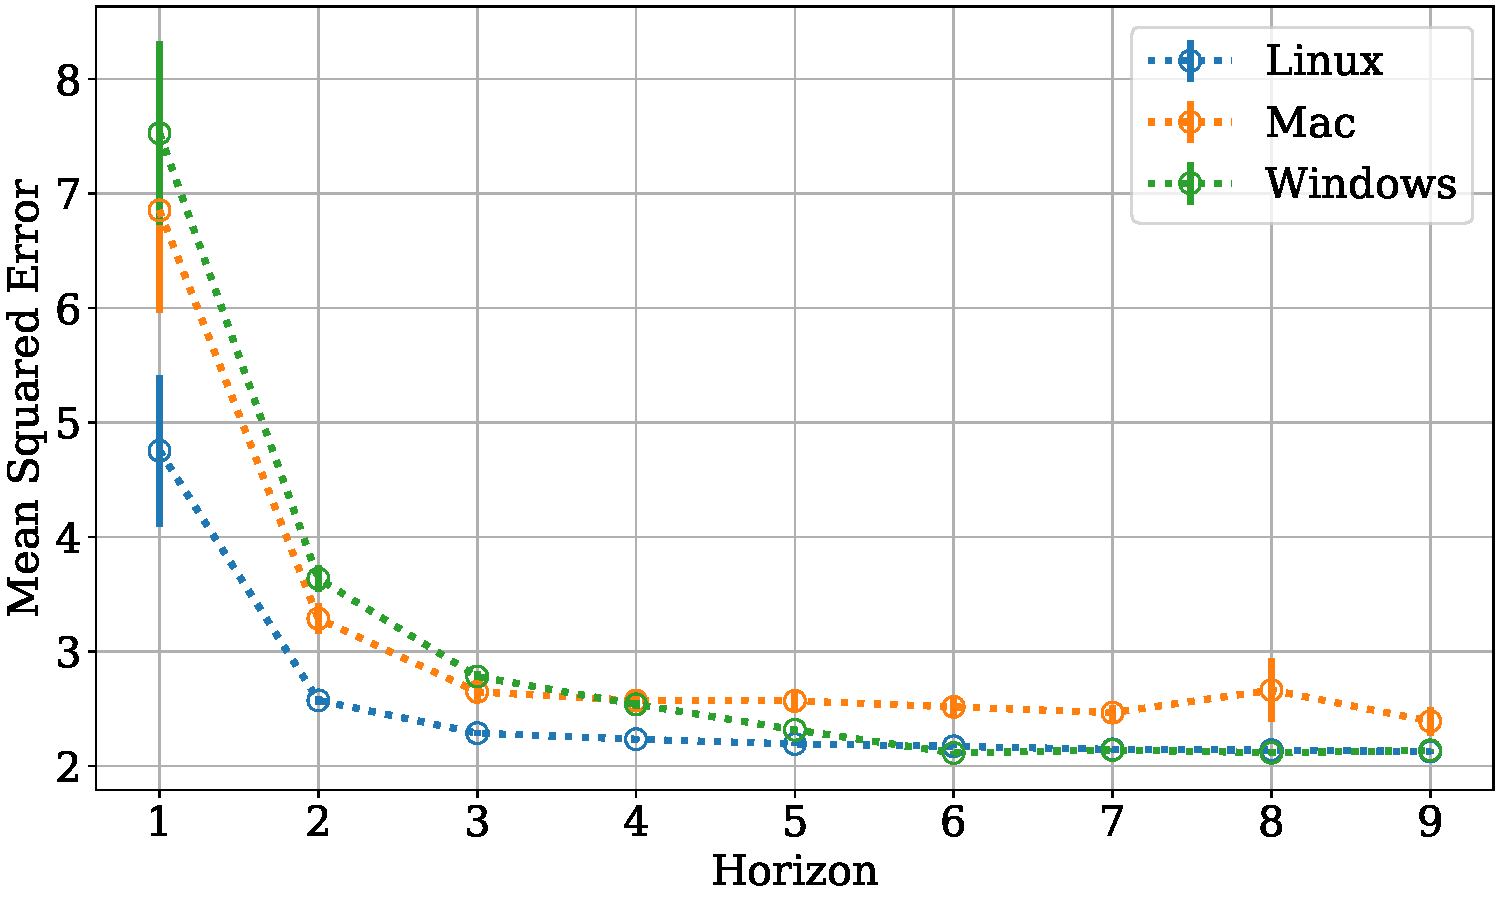
\includegraphics[width=\textwidth]{OS_MSE_against_H} 
    \caption{Network average estimation error $\overline{MSE}$}
    \label{fig:osmse}
  \end{subfigure}
  \hfill
  \begin{subfigure}[b]{0.49\textwidth}
    \centering
    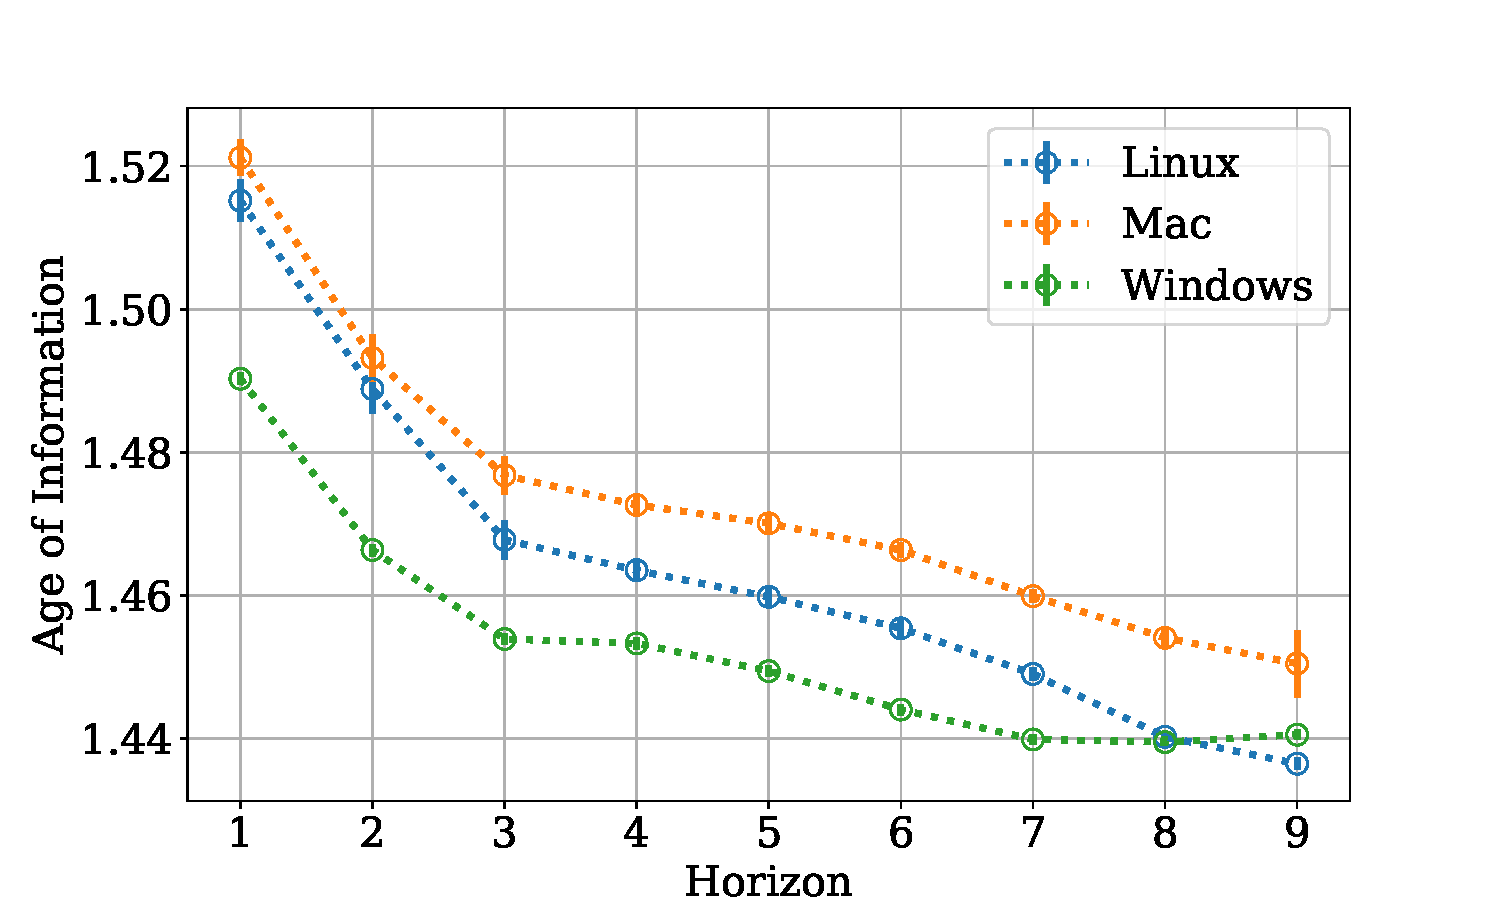
\includegraphics[width=\textwidth]{OS_AoI_against_H} 
    \caption{Network average AoI $\overline{\Delta}$}
  \end{subfigure}
  \caption[Comparison of network average MSE and AoI for different OS]{The two
  plots show $\overline{MSE}$ and $\overline{\Delta}$ for 200 simulation
  repetitions on Linux, Mac and Windows. Vertical error bars represent 95\%
  confidence intervals.}
  \label{fig:observation}
\end{figure}

Possible reasons for different OS behavior can root from either the algorithm or
its runtime implementation. From the algorithm's point of view MSE is influenced
by the quality of estimations, which are governed by information freshness,
i.e., AoI. In contrast, AoI is solely dependent on network outcome, which is
dependent on the scheduling decisions made at each time slot and the packet loss
process. The outcome of packet transmission may vary between OSs if their random
number generators differ. Regardless of algorithm design, the amount of
precision provided by arithmetic operations can also cause the observed
deviating numerical values. Other possible reasons may lie in machine runtime
levels. That is, before our simulation can run on a computing environment, a
compiler translates our simulation code into corresponding machine instructions
to be executed on the underlying hardware. A different machine instruction
implementation can also produce numerical inaccuracies affecting the algorithm's
behavior. Note that a thorough analysis on these lower abstraction levels are
beyond the scope of this thesis.

\footnotetext{The source code is available at \url{https://github.com/oayan/finite_horizon_scheduling}}

\section{Numerical Experimentation} \label{sec:experiments}

Taking aforementioned relationships into account, we suspect varying randomness
and/or numerical deviations, causing inconsistent scheduling policies, to be the
reason behind observed $\overline{MSE}$ and $\overline{\Delta}$. Hence, the
following investigation focuses on these two aspects.

\subsection{Random Number Generator}

Since computers are designed as deterministic machines, generating random
numbers on a computer forms a contradiction. Nevertheless, in modern computing,
deterministic random bit generators are used to cope with this problem. Instead
of true random numbers, these algorithms generate ``pseudo-random'' numbers
whose properties approximate true random numbers. A prominent example is a
\textit{Mersenne Twister} generator. Pseudorandomness is caused by the initial
value, also called \textit{seed}, given to the random number generator. In
particular, the output numbers are completely determined by the seed. Therefore,
it is important to initialize random number generators with unique seeds, e.g.
hardware state information. Further, the obtained raw numbers are transformed to
a suitable distribution for deployment.

\begin{figure}[htbp]
  \centering
  \begin{subfigure}[b]{0.49\textwidth}
      \centering
      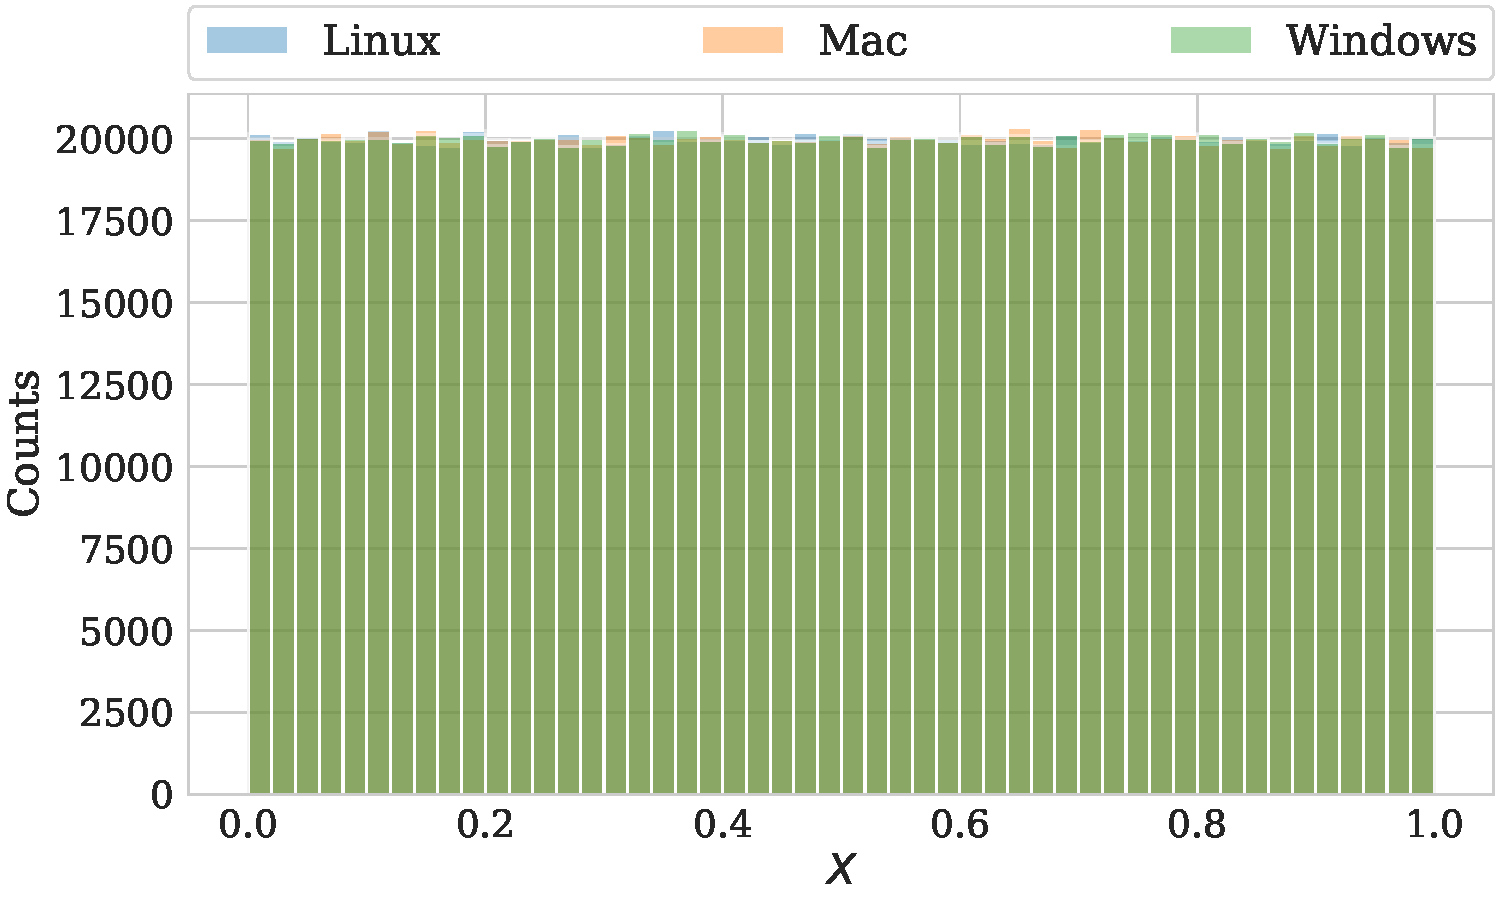
\includegraphics[width=\textwidth]{uniform}
      \caption{$X \sim \mathcal{N}(0.5, 0.2)$}
  \end{subfigure}
  \hfill
  \begin{subfigure}[b]{0.49\textwidth}
      \centering
      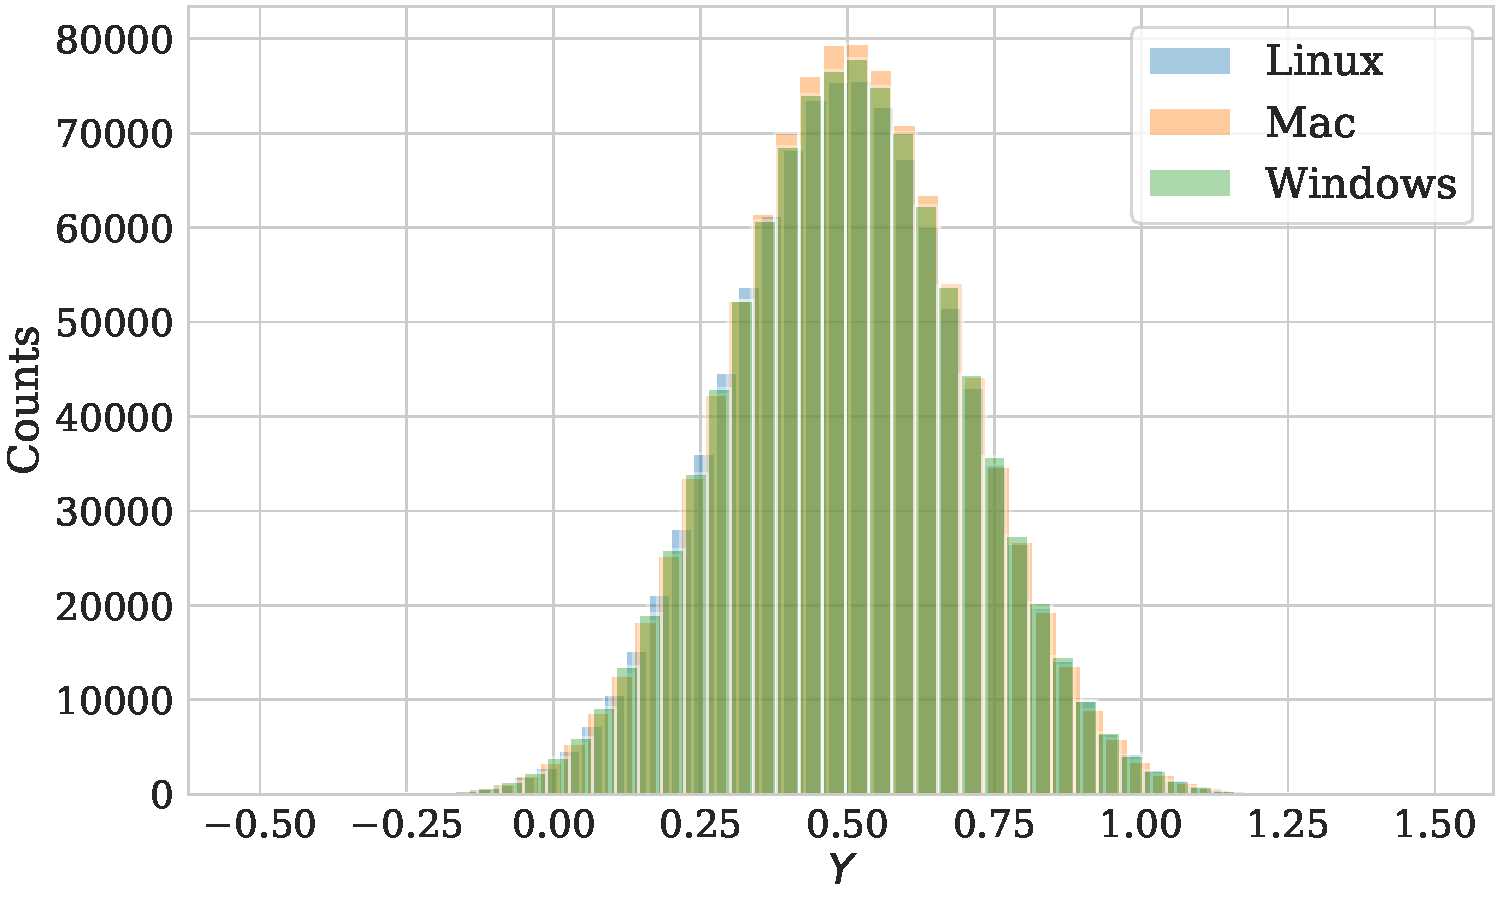
\includegraphics[width=\textwidth]{normal}
      \caption{$Y \sim \mathcal{U}(0, 1)$}
  \end{subfigure}
    \caption{The histograms of 1 million realizations of random variables utilized in simulations on Linux, Mac and Windows.}
    \label{fig:randomCheck}
\end{figure}

The employed NCS simulation framework determines system noise of sub-systems, GE
channel state transitions, as well as the outcome of packet transmissions from
Bernoulli experiments. The C++ standard library provides implementations for
both random engines and random number distributions. In our case, we have used
\texttt{std::default\_random\_engine} as random number generator and seed it
with the system clock count. As the simulations utilize normal and uniform
distributions, we have generated realizations of respectively distributed random
variables $X, Y$ on all tested OSs. Fig.~\ref{fig:randomCheck} depicts the
histogram of a million realizations each. It is visible, that the random number
generator performs consistent on all three platforms.

\subsection{Numerical effects on Scheduler}

Scheduling decisions are formed by the action which achieves minimal expected
cost as defined in Eq.~\eqref{eq:minimizationproblem}. To do so, the scheduler
maps measured AoI to an age-penalty following Eq.~\eqref{eq:gfunction}. In the
used NCS simulation framework, the scheduler initializes a \textit{cost map} at
each simulation run, which contains precomputed age-penalties until a predefined
maximum AoI for every simulated sub-system. The FHS employs these age-penalties
in a tree structure to perform combinatorial optimization by weighing possible
future nodes according to their occurrence in the tree. Numerical
inconsistencies in both cost maps and tree structures can cause different
schedules to be taken.

\begin{figure}[htbp]
  \centering
  \begin{subfigure}[b]{0.49\textwidth}
      \centering
      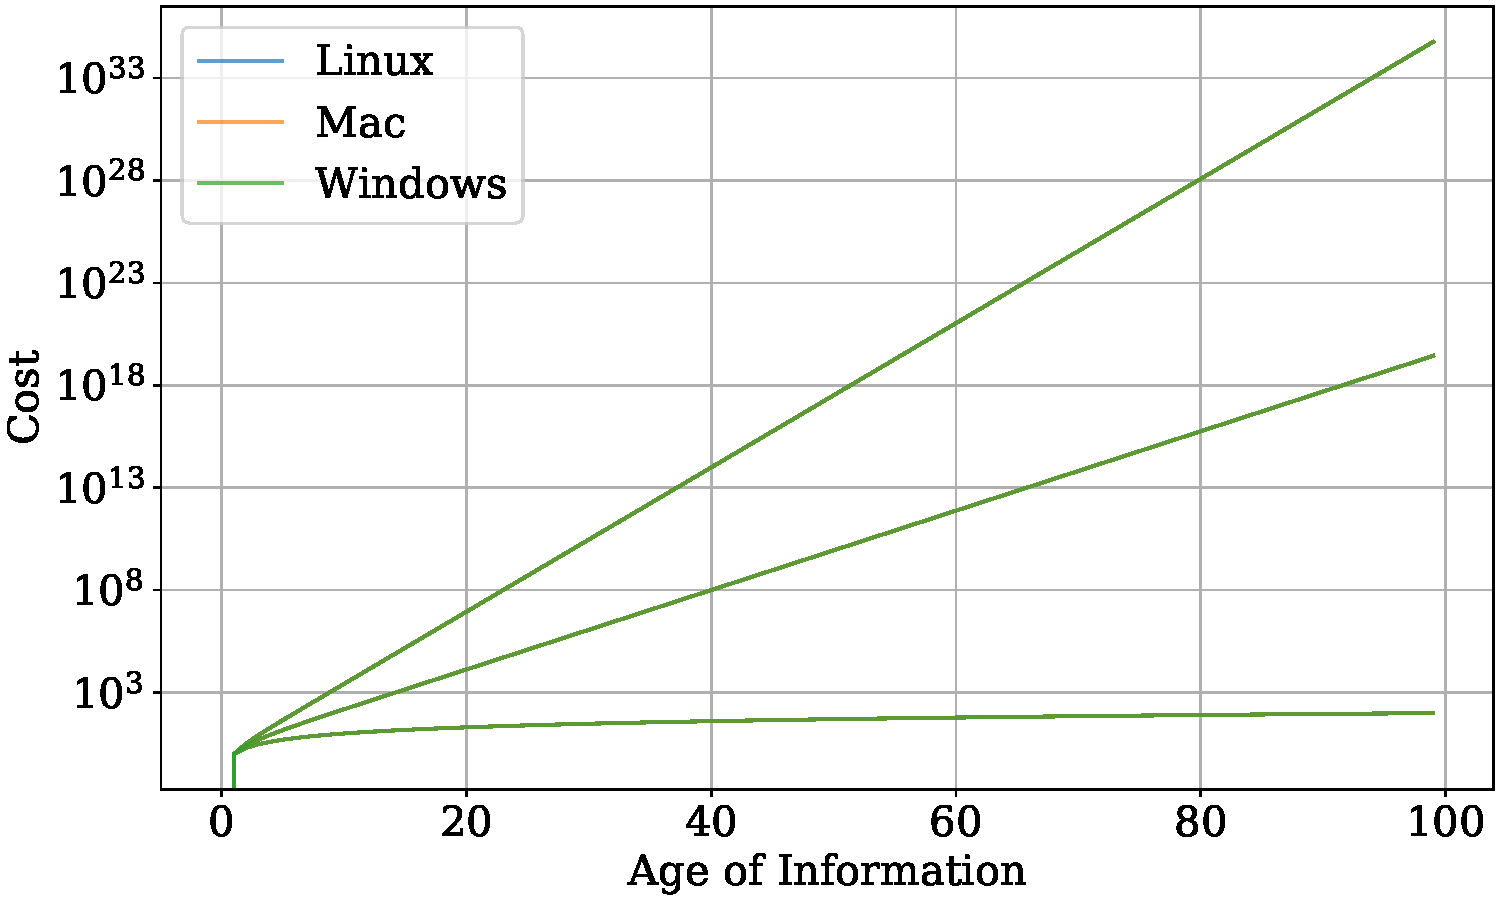
\includegraphics[width=\textwidth]{costMaps}
      \caption{Cost maps of FHS}
      \label{fig:costMaps}
  \end{subfigure}
  \hfill
  \begin{subfigure}[b]{0.49\textwidth}
      \centering
      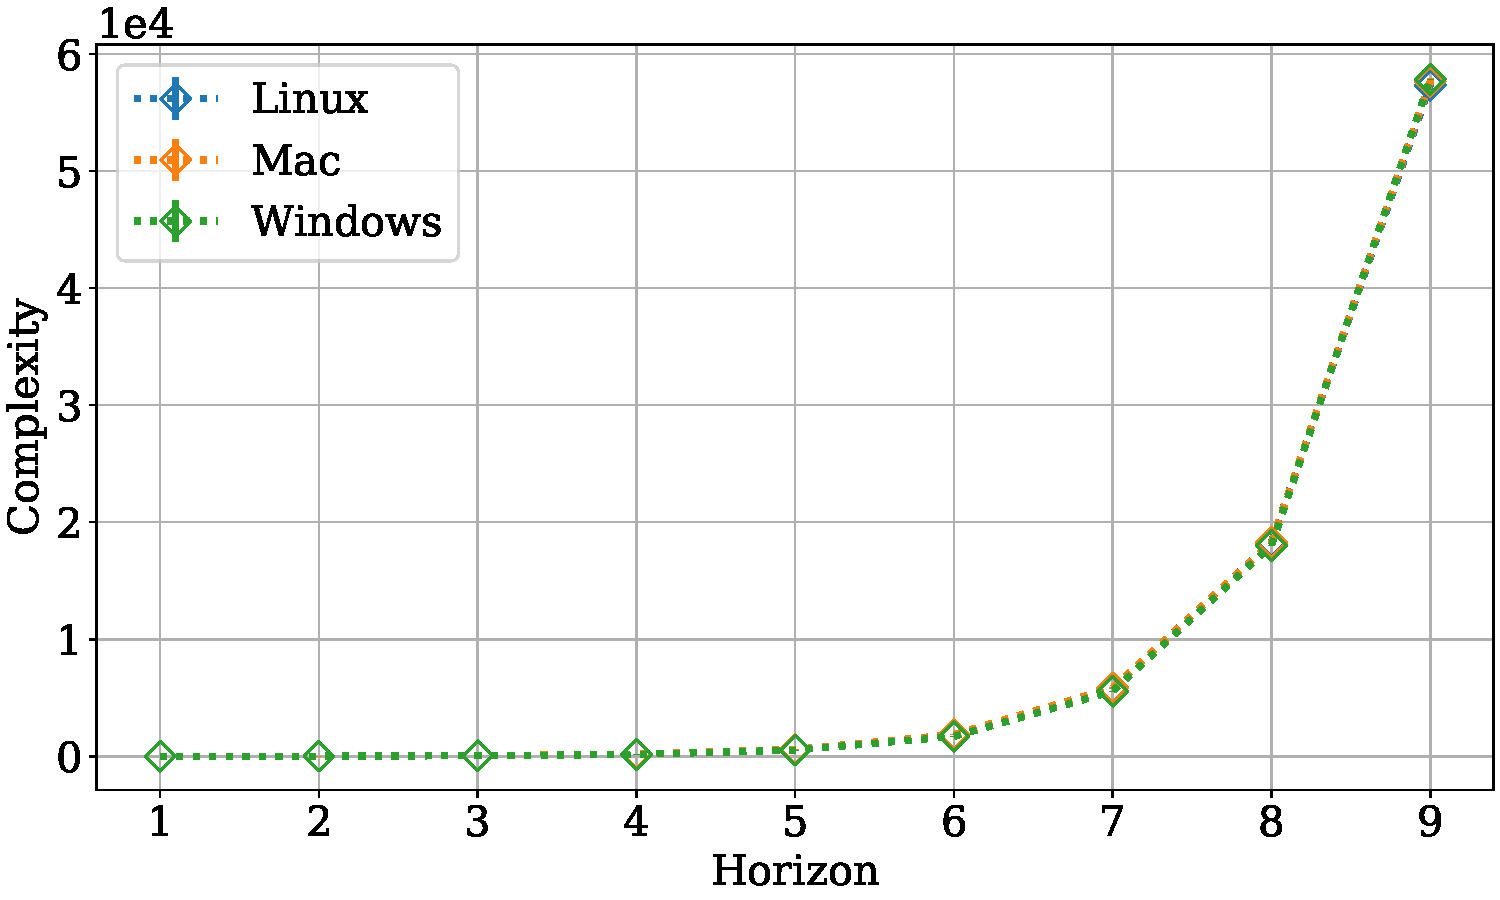
\includegraphics[width=\textwidth]{OS_AvgNodeCount_against_H}
      \caption{Average size of FHS tree}
      \label{fig:treesize}
  \end{subfigure}
    \caption[Comparison of FHS cost maps and average tree size for different
    OS]{The FHS cost maps and average tree size for Linux, Mac and Windows.}
\end{figure}

Fig.~\ref{fig:costMaps} depicts the cost maps of FHS for our considered test
scenario on different OSs. Note that, a cost map for $N=3$ consists of three
branches. We observe the same precomputed costs among Linux, Mac and Windows.
Furthermore, from Fig.~\ref{fig:treesize} it becomes evident that the average
tree size are identical for all OSs, meaning optimizations are performed on
identical trees. 

\subsection{Discussion}

The conducted numerical experimentation proves that our suspicions were wrong.
Neither different random number generators nor numerical inconsistencies in the
FHS algorithm were found. In addition, the changing Windows $\overline{MSE}$
trajectory seen in Fig.~\ref{fig:osmse} discharges different randomness as a
source for our observation. Otherwise, the trajectory should rather stay
consistently deviated and not switch between following Mac and Linux
trajectories. In the end, the reason behind the source of different simulation
results could not be clarified in this work. We have however proven that our
algorithm design is not a cause of our observation. As mentioned in Sec.
\ref{sec:effect}, different precision in floating point operations may cause the
deviating $\overline{MSE}$ and $\overline{\Delta}$ measurements. A further
investigation can be put in possible rounding errors caused by non-standard
implementations of floating point operations on Linux, Mac and Windows.
